\chapter{In-depth component description}

\section{Communicating with Channels}
\label{sec:channel}

\texttt{Channel} is an interface for performing I/O operations. It represents
the principal abstraction used by the middleware to communicate with hardware
devices and external software services.

\lstset{language=Java}
\begin{lstlisting}[float,caption=The Channel interface,label={lst:channel}]
public interface Channel {

	public String getId();
	
	public IOTask submit(IORequest request, IOHandler handler)
			throws ChannelException;
	
	public void setAsyncIOHandler(IOHandler handler)
			throws IllegalStateException;
			
	public boolean isClosed();
	
	public void close();
			
}
\end{lstlisting}

The \texttt{Channel} interface is not tied to any specific technology or
communication stack; as a result of this design choice, a wide variety of data
management tasks, including but not limited to, networking, file handling, and
automatic data generation can be implemented as \texttt{Channel}s.

The current Middleware architecture encourages the creation of several highly
specialized \texttt{Channel}s, which are usually developed around third-party
communication libraries. \texttt{HTTPChannel}, a \texttt{Channel} providing
support for HTTP communications, is an excellent example of the advantages of
this design strategy. Implemented as a simple wrapper around Apache's HTTP
Components toolkit, its development only required a basic understanding of the
HTTP protocol; yet \texttt{HTTPChannel} is a fully compliant HTTP/1.1 client
(see section~\ref{sec:channel.implementations} for additional details).

Upon instantiation, \texttt{Channel}s are open and ready to be used. They may
be optionally closed to relinquish unused resources by invoking the
\texttt{close()} method. Once closed, a \texttt{Channel} cannot be re-opened,
and every subsequent attempt to perform an I/O operation will fail causing a
\texttt{ChannelException} to be thrown. The current state of a \texttt{Channel}
can be probed through its \texttt{isClosed()} method.

Bytes sent or received with a \texttt{Channel} are encapsulated in a
\texttt{Payload} object. As shown in listing~\ref{lst:payload}, the
\texttt{Payload} interface allows all Middleware components to handle different
data types with a common set of methods, regardless of their individual
encoding.  \texttt{Payload}s will be the subject of further discussion in
section~\ref{sec:components.mapper}

\lstset{language=Java}
\begin{lstlisting}[float,caption=The Payload interface,label={lst:payload}]
public interface Payload {

	public Charset getCharset();

	public InputStream asInputStream();

	public ByteBuffer asByteBuffer();

	public String asString();

}
\end{lstlisting}

All user-initiated I/O operations begin with an invocation of the
\texttt{Channel.submit()} method. As can be seen in listing~\ref{lst:channel},
\texttt{submit()} is a direct implementation of the asynchronous interaction
paradigm introduced in section~\ref{sec:newmiddleware.async}. The emphasis on
asynchronous execution is underscored by the absence of blocking operations in
the \texttt{Channel} interface. This aspect is of paramount importance for the
entire Middleware design, as implementing a truly asynchronous system would
prove impossible if such feature were not provided by its core data access
layer.


\subsection{Instantiating new Channels}

\texttt{Channel}s are created by means of the \texttt{ChannelFactory}
interface, a reification of the Factory design pattern that allows polymorphic
instantiation of new object classes.

By using a Factory instantiation model, the choice of a particular
\texttt{Channel} implementation can be postponed from compile time to run time.
This technique allows the Middleware to dynamically adapt in response to
environment changes, and to support extension through the addition of new
user-defined \texttt{Channel}s. For further information regarding the Factory
pattern and its other uses inside the PerLa Middleware, refer to
section~\ref{sec:newmiddleware.factory}.

All the information required to create a new \texttt{Channel} is stored inside
a \texttt{ChannelDescriptor}. As shown in listing~\ref{lst:channelFactory},
this configuration object is the only parameter required to correctly invoke
the \texttt{createChannel()} method.

\lstset{language=Java}
\begin{lstlisting}[float,caption=The ChannelFactory
interface,label={lst:channelFactory}]
public interface ChannelFactory {

	public Class<? extends ChannelDescriptor>
			acceptedChannelDescriptorClass();

	public Channel createChannel(ChannelDescriptor descriptor)
			throws InvalidDeviceDescriptorException;

}
\end{lstlisting}

\begin{figure}[h!]
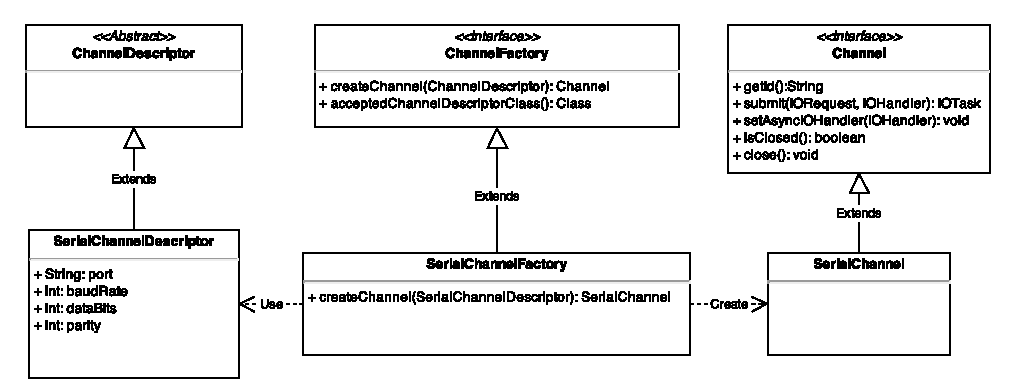
\includegraphics[width=\textwidth]{imgs/channel_factory.pdf}
\caption{Class diagram of the Channel layer}
\end{figure}

Each \texttt{ChannelFactory} is tied to a specific communication technology;
therefore, it can only accept a single class of \texttt{ChannelDescriptor}
objects. For example, the \texttt{HTTPChannelFactory} parses
\texttt{HTTPChannelDescriptor}s and creates \texttt{HTTPChannel}s, whereas an
hypothetical \texttt{SerialChannelFactory} would consume
\texttt{SerialChannelDescriptor}s to create \texttt{SerialChannel}s. Failure to
provide a suitable \texttt{ChannelDescriptor} object will cause the
\texttt{createChannel()} method to throw an
\texttt{InvalidDeviceDescriptorException}.

The \texttt{acceptedChannelDescriptorClass()} method can be used to dynamically
discover which \texttt{ChannelDescriptor} type is supported by a specific
\texttt{ChannelFactory}. This method is the fulcrum of the \texttt{Channel}
Plugin System, as it allows the Middleware to invoke the most appropriate
\texttt{ChannelFactory} using only information available at runtime.

\begin{figure}[!hbt]
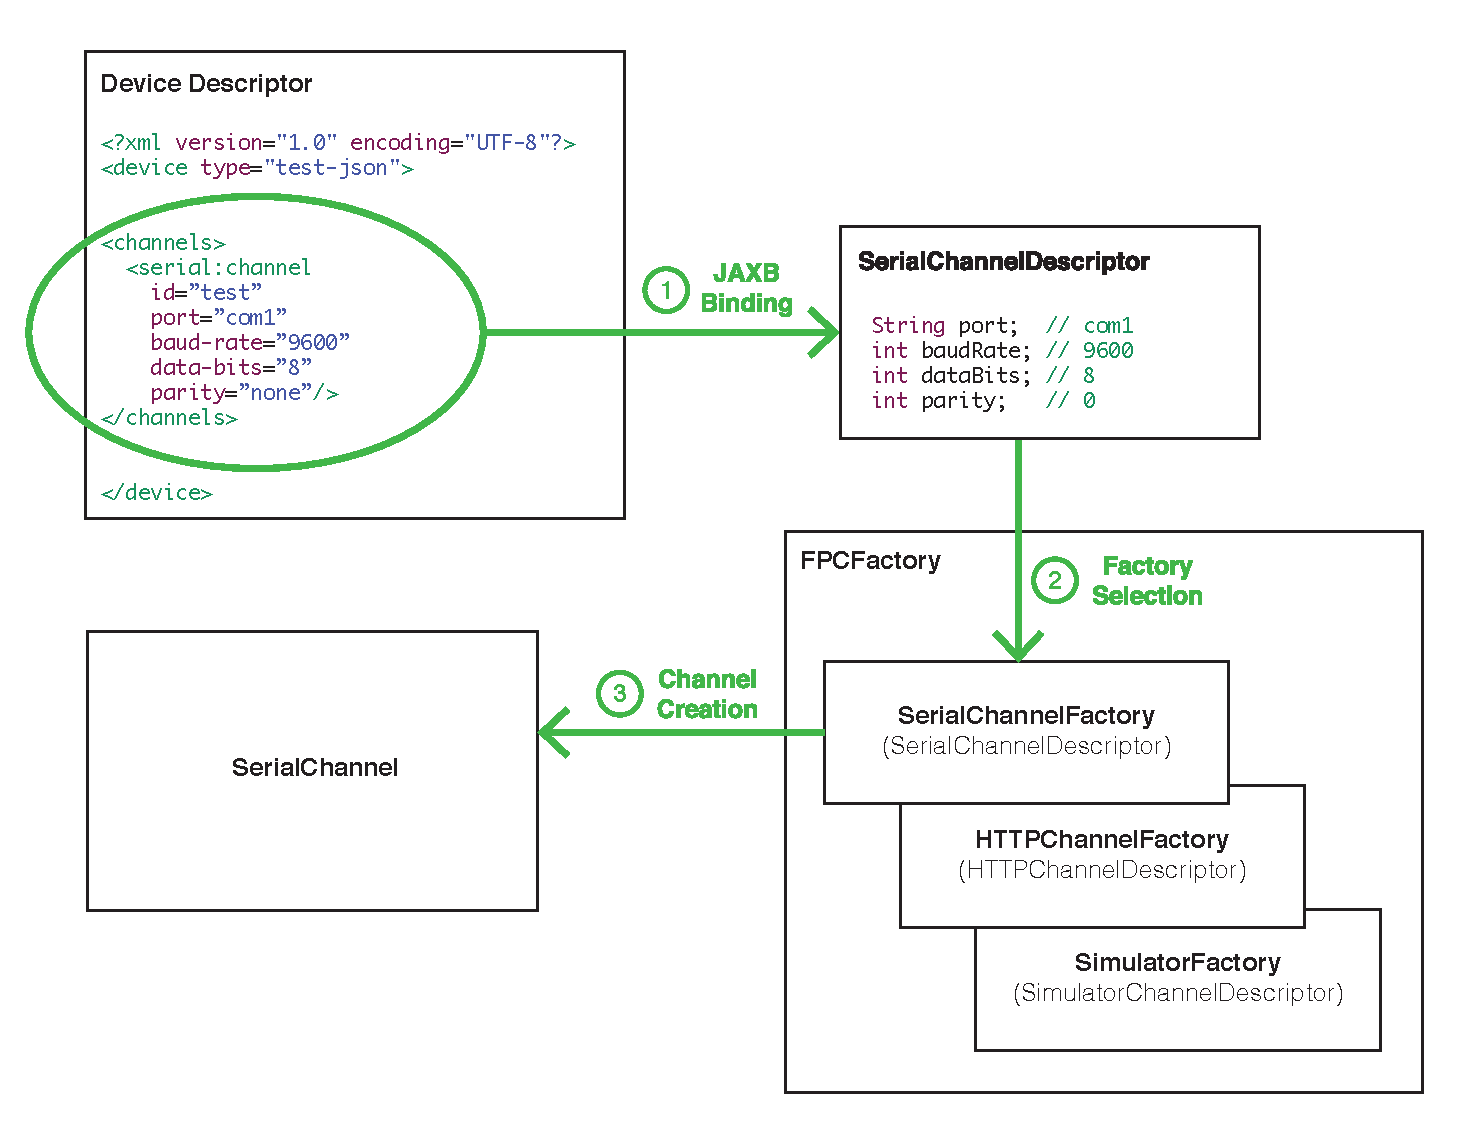
\includegraphics[width=\textwidth]{imgs/channel_creation_process.pdf}
\caption{The Channel creation process}
\label{fig:channel.creation}
{
\begin{figurenote}
This figure illustrates the \texttt{Channel} creation process executed by the
Middleware upon reception of a new Device Descriptor.  \begin{enumerate}
  \itemsep0em
  \item JAXB binds the XML Device Descriptor to an apropriate
\texttt{ChannelDescriptor} object using namespace information \item A suitable
\texttt{ChannelFactory} is selected at runtime using the
\texttt{acceptedChannelDescriptorClass()} method
  \item The information contained in the \texttt{SerialChannelDescriptor} is
used to create a new \texttt{SerialChannel} \end{enumerate}
\end{figurenote}
}
\end{figure}

\texttt{ChannelDescriptor} objects are automatically created by the
Middleware using the information contained in the Device Descriptor XML files.
This binding process is performed by the JAXB library, which is also
responsible for instantiating the correct \texttt{ChannelDescriptor} class
using XML Namespace information. Figure~\ref{fig:channel.creation} illustrates
this technique, and ties it together with the other operations described in
this section.

It is important to note that a single JVM instance running the PerLa Middleware
may host several \texttt{Channel} objects of the same type, at the same time.
Several devices can use the same communication technology, and the
\texttt{ChannelFactory} may determine that it's best to create an individual
\texttt{Channel} for each one of them. This behaviour is fostered by the new
\texttt{ChannelFactory} architecture, and is considered idiomatic design;
hence, it would not be uncommon to implement the hypothetical
\texttt{SerialChannelFactory} introduced in the previous paragraphs so that
every serial port is handled by a different \texttt{SerialChannel} instance.


\subsection{IORequest management}

\texttt{IORequest} is the base object interface employed to interact with a
sensing node connected to the Middleware. It contains two types of information:
the payload to be transferred, and \texttt{Channel}-dependent data needed for a
correct communication with the endpoint device.

\lstset{language=Java}
\begin{lstlisting}[float,floatplacement=!hbt,caption=The IORequest
interface,label={lst:iorequest}]
public interface IORequest {

	public String getId();

	public void setParameter(String name, Payload payload);
	
}
\end{lstlisting}

Every \texttt{Channel} imlementation is bundled with its own custom
\texttt{IORequest} class. Following up on previous examples, the
\texttt{HTTPChannel} package contains a \texttt{HTTPIORequest} object, whereas
the fictitious \texttt{SerialChannel} would be supplied with a
\texttt{SerialIORequest} class of request objects. This additional level of
indirection is necessary since different communication technologies require
different settings to establish end-to-end connectivity; therefore, a universal
\texttt{IORequest} object would soon prove to be a limiting factor for the
extension of the Middleware.

As shown in listing~\ref{lst:iorequest}, payload data can be set in an
\texttt{IORequest} by means of the \texttt{setParameter()} method.
\texttt{Payload}s are addressed by name, and a single \texttt{IORequest}
implementation may support several at once. The exact set of \texttt{Payload}
parameters accepted by an \texttt{IORequest} class depends on the design of its
matching \texttt{Channel}; for example, the \texttt{HTTPChannel}
implementation supports three: an `entity' payload (request body), a `query'
payload (an URL-encoded string), and a `path' payload (a path component used to
identify a single resource accessible from the base URL).

\texttt{IORequest}s are disposable objects; they are created, submitted to a
\texttt{Channel}, and garbage collected once the communication is over.
Creation is performed by means of a factory interface dubbed
\texttt{IORequestBuilder}, which allows the Middleware to build new copies of
an \texttt{IORequest} from a fixed template. It is important to note that
request objects built using this technique do not contain \texttt{Payload}
parameters; these are to be added manually before subbmitting the
\texttt{IORequest} to a \texttt{Channel}.

Besides \texttt{IORequest} creation, the \texttt{IORequestBuilder} interface
can be used to dynamically discover which \texttt{Payload} parameters are
supported by an \texttt{IORequest}. This functionality, exposed through the
\texttt{getParameterList()} method, is a crucial component of the Middleware
Plugin System, as it allows \texttt{Script} instructions to determine whether
an \texttt{IORequest} was populated with all the necessary \texttt{Payload}
parameters or not. This concept will be the subject of further analysis in
section~\ref{sec:components.script}.

A single device connected to the PerLa Middleware is generally managed using
several \texttt{IORequestBuilder}s, any one of which is responsible for
creating a request object suitable to control a single aspect of
the interaction with the endpoint. The main advantage brought by this
templating mechanism is that \texttt{Channel}-related configuration settings
are only specified once, hence the same \texttt{IORequest} structure can be
reused multiple times to transport different payload information.

\lstset{language=Java}
\begin{lstlisting}[float,floatplacement=!hbt,caption=The IORequestBuilder
interface,label={lst:iorequestbuilder}]
public interface IORequestBuilder {

	public String getRequestId();

	public IORequest create();

	public abstract List<IORequestParameter> getParameterList();

	public static class IORequestParameter {

		public String getName() {
			return name;
		}

		public boolean isMandatory() {
			return mandatory;
		}

	}
}
\end{lstlisting}

REST APIs are an excellent use case to demonstrate the aforementioned concept,
as every operation on a RESTful resource can be easily abstracted using an
appropriately configured request builder. By using
\texttt{HTTPIORequestBuilder} objects, HTTP protocol information (base URL,
method, header, \ldots) are specified one single time only for
every REST endpoint. Once this step is done, the API can be invoked just by
building new \texttt{IORequest}s and submitting them to a \texttt{HTTPChannel}.

\begin{figure}[!hbt]
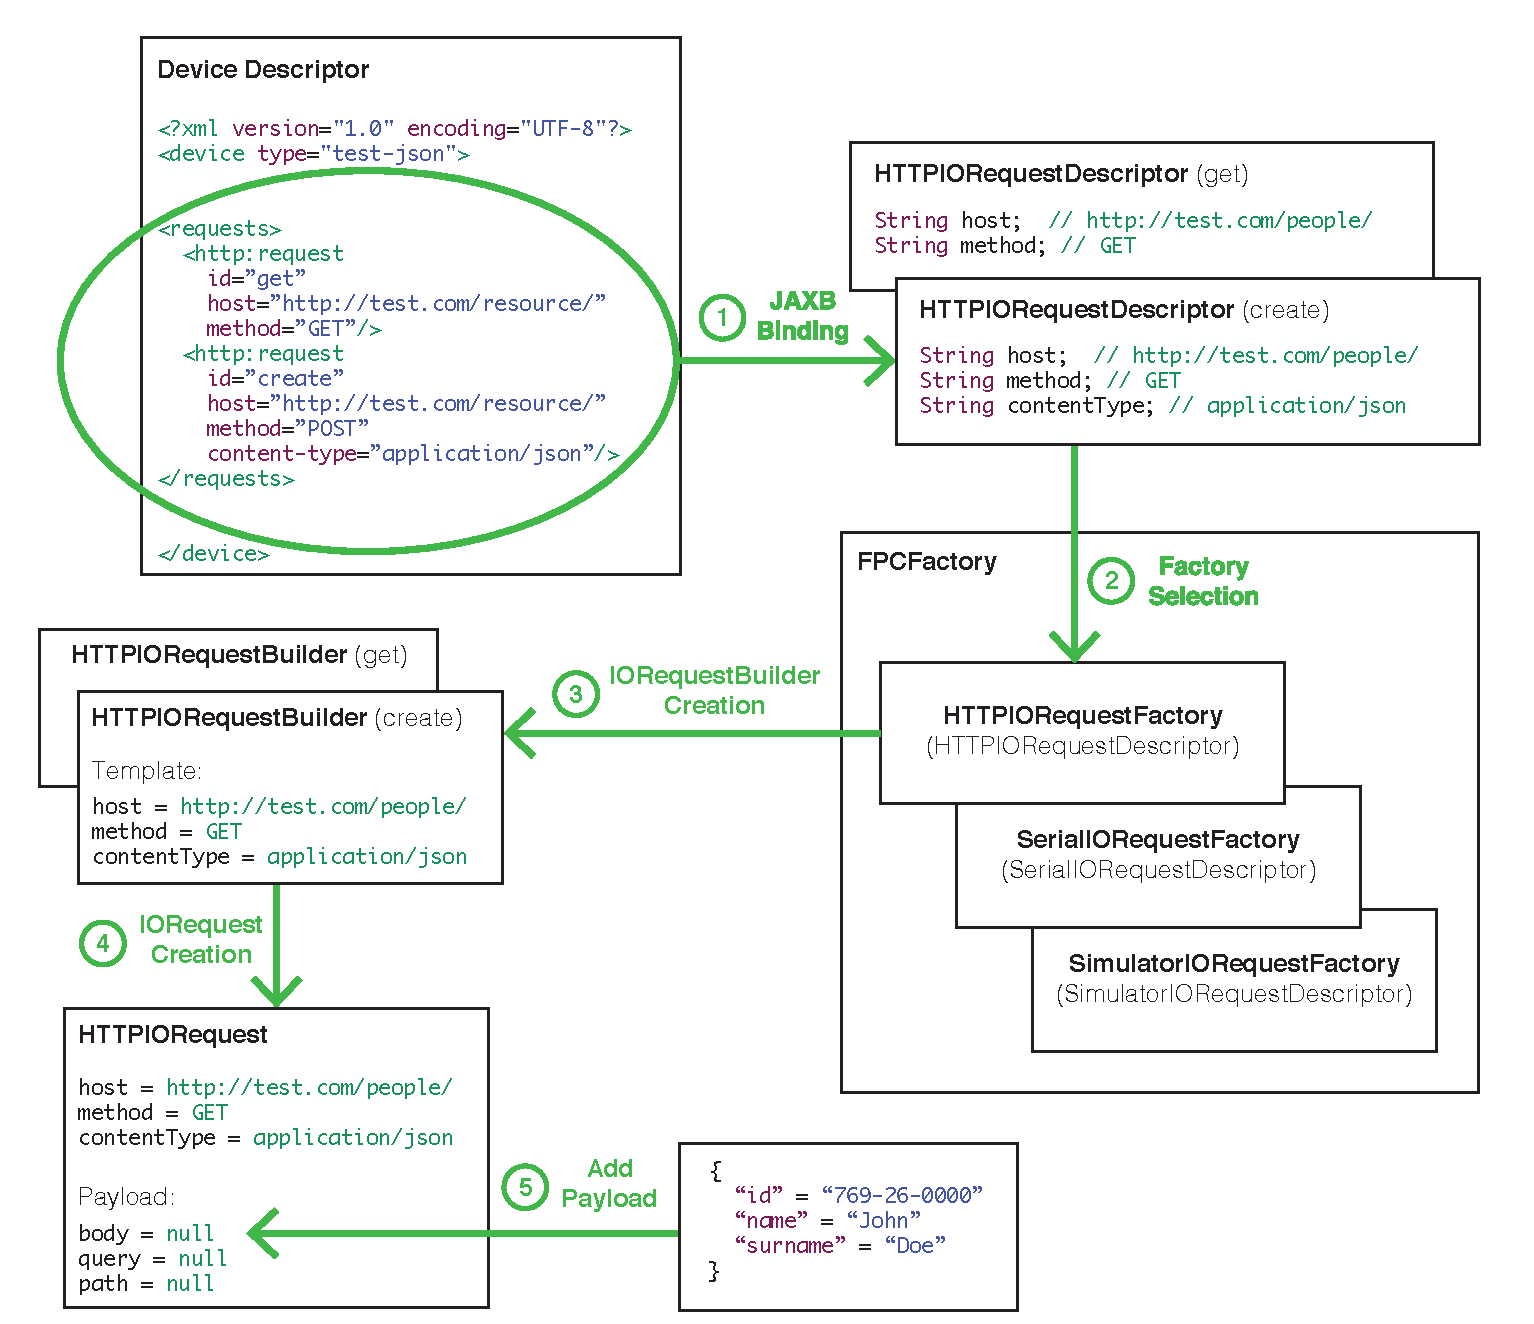
\includegraphics[width=\textwidth]{imgs/iorequest_creation_process.pdf}
\caption{The IORequest creation process}
\label{fig:iorequest.creation}
{
\begin{figurenote}
This figure illustrates the autonomous creation of \texttt{IORequest} objects.
Steps 1 to 3 are performed only once after receiving the Device Descriptor,
whereas steps 4 and 5 are repeated every time the REST API is to be invoked.
\begin{enumerate}
  \itemsep0em
  \item JAXB binds the XML Device Descriptor to an apropriate
\texttt{IORequestDescriptor} object using namespace information \item A
suitable \texttt{IORequestBuilderFactory} is selected at runtime using the
\texttt{acceptedIORequestDescriptorClass()} method
  \item The information contained in the \texttt{IORequestDescriptor} is used
to create a new \texttt{IORequestBuilder} \item The \texttt{IORequestBuilder}
is used to create new \texttt{IORequest} copies using the internal template
  \item The newly created \texttt{IORequest} objects can be populated with
\texttt{Payload} parameters as needed \end{enumerate}
\end{figurenote}
}
\end{figure}

\texttt{IORequestBuilder}s are created by means of an
\texttt{IORequestBuilderFactory}, an object that implements the now familiar
Factory design pattern. Creation proceeds as follows: the request template is
loaded from an XML Device Descriptor, bound to an appropriate
\texttt{IORequestDescriptor}, and processed by the
\texttt{IORequestBuilderFactory} to create the corresponding
\texttt{IORequestBuilder}. Similarly to what already seen in the previous
section, every \texttt{IORequestBuilderFactory} implements an
\texttt{acceptedIORequestDescriptorClass()} method, which can be used to
dynamically determine if a factory object can parse a specific type of
\texttt{IORequestDescriptor}. It should come as no surprise that every
\texttt{IORequestBuilder} class is provided with complementary
\texttt{IORequestBuilderFactory} and \texttt{IORequestDescriptor}
implementations.

\begin{figure}[!hbt]
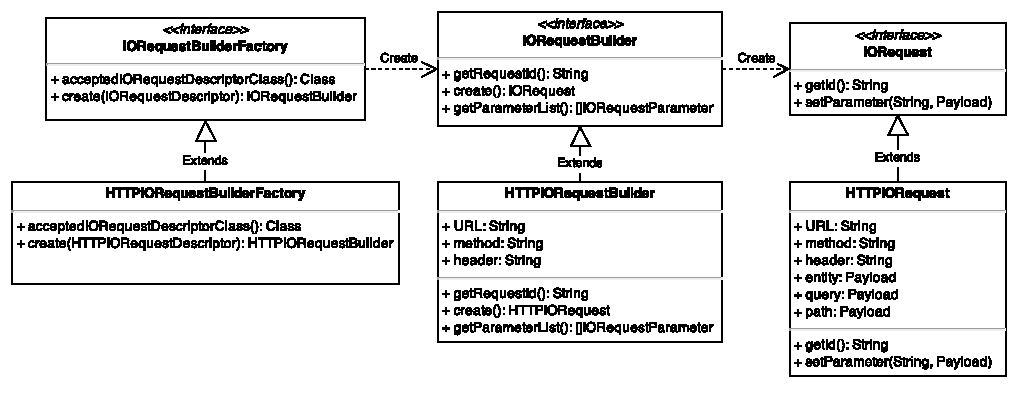
\includegraphics[width=\textwidth]{imgs/iorequest.pdf}
\caption{The extended IORequest class diagram. For additional information about
the IORequestParameter object consult listing 1.5.} \label{fig:iorequest.class}
\end{figure}


\subsection{Handling asynchronous I/O operations}

As mentioned in previous sections, communication with a device connected to the
PerLa Middleware is achieved by means of the \texttt{Channel.submit()} method.
Invocations of \texttt{submit()} are non-blocking; control flow is immediately
returned to the caller, thus allowing other computations to be performed while
the requested I/O operation is being processed.

As can be seen in listing~\ref{lst:channel}, \texttt{submit()} requires two
parameters: an \texttt{IORequest} and an \texttt{IOHandler} callback object.
The former specifies which I/O operation is to be performed, while the latter
allows the caller to be asynchronously notified of its completion.

The \texttt{IOHandler} interface is composed of two methods, namely
\texttt{complete()} and \texttt{error()}, which are invoked when processing of
an I/O operation comes to an end. It is important to note that both these
methods always carry context information in the form of an \texttt{IORequest},
which is guaranteed to be the same exact object used for starting the I/O
operation whose completion is being notified. For this reason,
\texttt{IOHandler} can be considered the nexus of the asynchronous invocation
model, as it connects \texttt{IORequest} objects with the outcome of the
corresponding I/O operation performed by the \texttt{Channel}.

\lstset{language=Java}
\begin{lstlisting}[float,floatplacement=H,caption=The IOHandler
interface,label={lst:iohandler}]
public interface IOHandler {
	public void complete(IORequest request, Optional<Payload> result);
	
	public void error(IORequest request, Throwable cause);
}
\end{lstlisting}

\lstset{language=Java}
\begin{lstlisting}[float,floatplacement=!hbt,caption=The IOTask
interface,label={lst:iotask}]
public interface IOTask {
	public void cancel();
	
	public IORequest getRequest();
	
	public boolean isCancelled();
	
	public boolean isDone();
}
\end{lstlisting}

Semantically, an invocation of the \texttt{complete()} method is always
associated with the successful termination of an I/O operation. As shown in
listing~\ref{lst:iohandler}, this method includes an optional \texttt{Payload}
object, that contains all data received from the endpoint device. A call to
\texttt{complete()} with an empty \texttt{Payload} indicates that the I/O
operation was completed without errors, but no data was received. Conversely,
an invocation of the \texttt{error()} method indicates that the I/O operation
was aborted before completion. In this case the cause of failure is always
notified through the \texttt{cause} parameter.

From the point of view the Java memory model, the \texttt{Channel.submit()}
creates a happens-before relationship with \texttt{IOHandler.complete()} and
\texttt{IOHandler.error()}, viz. any side effect generated by the code that led
to the \texttt{submit()} invocation is guaranteed to be visible in the
\texttt{complete()} and \texttt{error()} callback methods.

Asynchrous execution does not imply loss of control; ongoing I/O operations can
be monitored or cancelled by means of the \texttt{IOTask} object acquired upon
submitting an \texttt{IORequest}. Listing~\ref{lst:iotask} shows all methods of
the \texttt{IOTask} interface; method names are self explanatory, and the
reader should be able to deduce their purpose just by analyzing their 
signature. The only nuance worth mentioning is that
\texttt{isCancelled()} always implies \texttt{isDone()} (i.e., all cancelled
I/O operations are also complete), while the opposite does not hold (i.e., not
all complete I/O operations were cancelled).

\begin{figure}[!hbt]
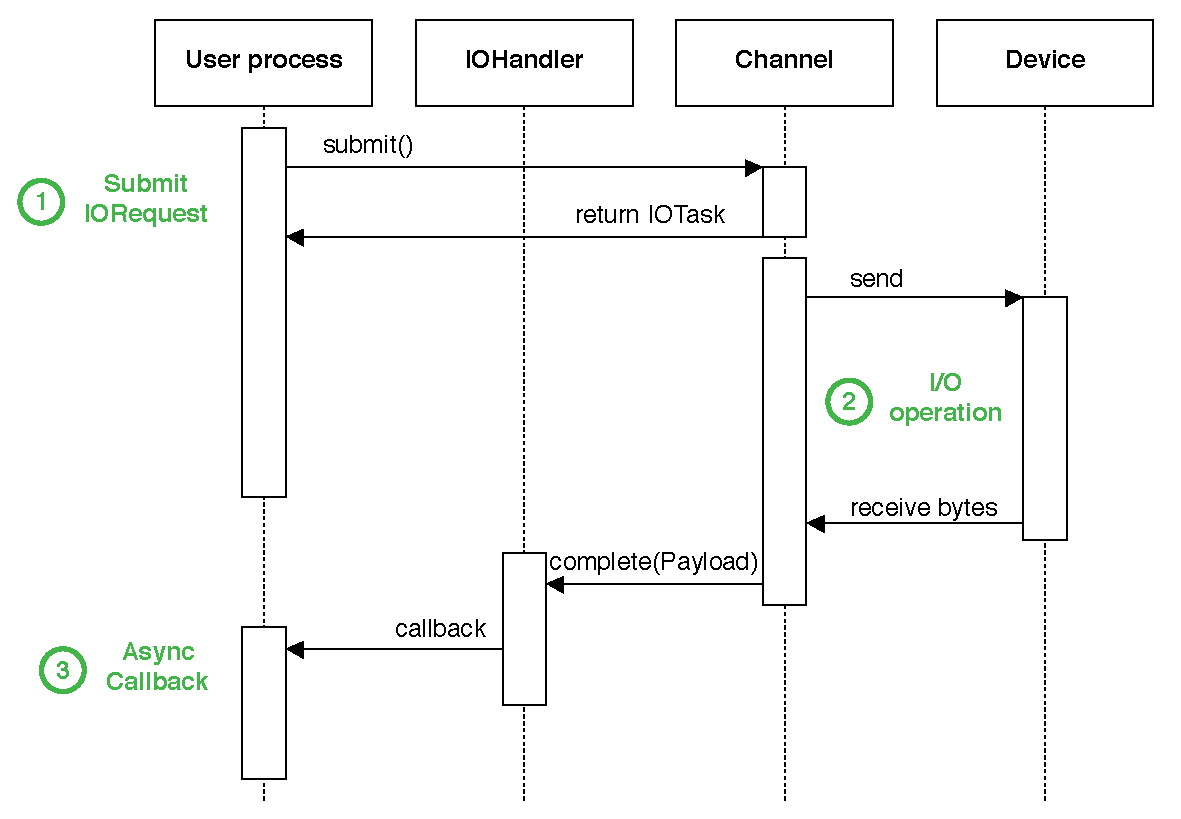
\includegraphics[width=\textwidth]{imgs/async_channel_sequence.pdf}
\caption{Sequence diagram of an asynchronous I/O operation. Note that the user
process and the I/O operation are executed in parallel.}
\label{fig:channel.async}
\end{figure}

The \texttt{Channel} interface is also designed to manage completely
asynchronous I/O operations, namely communication efforts spontaneously
initiated by the remote device. This communication model is popular among WSNs,
as it is often employed to handle periodic data streams or events happening
at irregular intervals. Such I/O operations can be handled through a catch-all
\texttt{IOHandler} set with the \texttt{setAsyncIOHandler()} method
(listing~\ref{lst:channel}). Since the communication is not initiated by the
Middleware, the \texttt{complete()} and \texttt{error()} callback methods will
be invoked with the \texttt{IORequest} parameter set to \texttt{null}.


\section{Handling data}
\label{sec:components.mapper}

\texttt{Payload} is a container for raw sequences of bytes. In spite of its
semplicity, this class forms the foundation of the entire PerLa Middleware, as
it is the vessel that conveys all information passing through the
\texttt{Channel} interface.

The data encapsulated in a \texttt{Payload} object is accessed one byte at a
time; this granularity level is ideal for the implemention of an I/O access
layer, whose sole concern consists in the transmission of information between
two endpoints, but is not suited to other forms of data management. Processing
the information contained in a \texttt{Payload} can be unwieldy and
unnecessarily complex; the byte-oriented interface doesn't provide any facility
for leveraging the underlying structure of the enclosed data, and even a simple
action like retrieving a value in a complex data structure can easily become a
daunting task.


\subsection{The Message interface}

\texttt{Message}s are structured data containers that enclose a group of
individual items called fields. The chief advantage that this data structure
provides over the simpler \texttt{Payload} object consists in the possibility
of addressing information by field name, a convenient feature that dispenses
with the burden of managing data in byte-sized chunks. The methods available in
the \texttt{Message} interface are shown in listing~\ref{lst:message}.

\lstset{language=Java}
\begin{lstlisting}[float,floatplacement=!hbt,caption=The Message
interface,label={lst:message}]
public interface Message {

    public String getType();

    public boolean hasField(String name);

    public Object getField(String name)
                throws IllegalArgumentException;

    public void setField(String name, Object value)
                throws IllegalArgumentException;

    public void appendElement(String name,Object element)
                throws IllegalArgumentException;

    public boolean validate();

}
\end{lstlisting}

The specific structure of a \texttt{Message} is defined by its type, which can
be queried through the \texttt{getType()} method. This property unequivocally
identifies the set of fields contained in a \texttt{Message} in terms of field
\textbf{name}, field \textbf{type} and field \textbf{qualifier}.

The field \textbf{name} is a textual attribute that uniquely identifies one
specific data item in the scope of a single \texttt{Message}. It can be used to
retrieve or set the value of a field through the \texttt{getField()} and
\texttt{setField()} methods respectively.

The \textbf{type} attribute defines the set of legal values that can be stored
in a field, together with the operations that are allowed on those values. It
is worth mentioning that this information is used to statically verify the type
safety of nearly all data management operations performed on a \texttt{Message}
(consult section~\ref{sec:components.script} for additional information). The
PerLa Middleware currently supports six primitive types:

\begin{itemize}

  \item \textbf{INTEGER}: a 32 bit signed two's complement integral data type

  \item \textbf{FLOAT}: a single-precision 32 bit IEEE 745 floating point

  \item \textbf{BOOLEAN}: a type with only two values, true or false

  \item \textbf{STRING}: a string of characters with UTF-16 encoding

  \item \textbf{TIMESTAMP}: a date with timezone, currently implemented using
      Java's \texttt{ZonedDateTime} class.

  \item \textbf{ID}: a unique label that identifies a single node connected in
      a PerLa managed network. The current implementation uses a 32 bit
      integer. 

\end{itemize}

Besides the data types presented above, fields can also be configured to hold
nested \texttt{Message}s. In this case, the type attribute must be set to the
particular type of \texttt{Message} that is to be stored in the field. 

The \textbf{qualifier} attribute is employed to define additional field
properties. It can be set to one of the following values:

\begin{itemize}

  \item \textbf{SIMPLE}: a normal field whose value can be altered and
      retrieved using the \texttt{setField()} and \texttt{getField()} methods
      respectively.

  \item \textbf{LIST}: a field that can hold multiple elements of the same
      type. New values can be added with the \texttt{appendElement()} method,
      and the entire list can be retrieved through the conventional
      \texttt{getField()} method. List-qualified fields preserve the order of
      insertion of the individual elements.

  \item \textbf{STATIC}: a field whose value is statically set when the
      \texttt{Message} type is declared. Any attempt to modify a
      statically-qualified field with either the \texttt{setField()} or the
      \texttt{appendElement()} methods will cause an exception to be thrown. It
      is important to note that static field values are set on a per-type
      basis; this means that all \texttt{Message}s of the same type will share
      the same field values for each static field (if any).
      
\end{itemize}


\subsection{Working with Messages: the Mapper interface}

\texttt{Message} objects are managed by the \texttt{Mapper} component. Its
interface, available in listing~\ref{lst:mapper}, groups all the
functionalities needed to handle a specific variety of structured information.
The one-to-one relationship between \texttt{Mapper}s and data types is
epitomized by the \texttt{getMessageType()} method, whose return value
indicates which \texttt{Message} class is supported by a particular
\texttt{Mapper}. This method is extensively employed by the Middleware to sift
through a collection of \texttt{Mapper}s, in order to find one that is best
suited for handling the information currently being processed.

\lstset{language=Java}
\begin{lstlisting}[float,floatplacement=!hbt,caption=The Mapper
interface,label={lst:mapper}]
public interface Mapper {

    public String getMessageType();

    public FieldDescriptor getFieldDescriptor(String name);

    public Collection<FieldDescriptor> getFieldDescriptors();

    public FpcMessage createMessage();

    public FpcMessage unmarshal(Payload payload);

    public Payload marshal(FpcMessage message);

}
\end{lstlisting}

Interactions with a \texttt{Mapper} usually begin with a call to the
\texttt{createMessage()} method, whose execution results in the creation of an
empty \texttt{Message} instance. Despite its unsuprising outcome, this method
draws once again our attention to the close relationship between
\texttt{Mapper}s and data types. Every \texttt{Mapper} instance is in fact
committed to the management of a precise class of information, hence all
\texttt{Message}s created with the \texttt{createMessage()} method will share
the same data type property, and, consequently, the same set of fields. The
interdependence between a \texttt{Mapper} and its assigned type is accentuated
even further by the \texttt{getFieldDescriptor()} and
\texttt{getFieldDescriptors()} methods, which can be used to analyze the
internal field structure characterizing all \texttt{Message} objects that the
\texttt{Mapper} creates. This introspective capability is extensively exploited
in the Execution Engine to check whether a \texttt{Script} is type-safe or not
(see section~\ref{sec:components.script} for further details).

As explained in the introductory paragraphs of this section, \texttt{Message}
objects are a convenience introduced for simplifying data management operations
in the PerLa Middleware. They provide structured access to information, a
familiar set of primitive data types, and a selection of tools for combining
basic values into complex data structures. In spite of these advantages, the
\texttt{Message} interface is a high level abstraction that cannot be employed
where a \texttt{Payload} is expected, since its contents are not directly
accessible as a simple sequence of bytes; as a consequence, \texttt{Message}s
can't be used for any kind of I/O operation. This structural gap is bridged by
the \texttt{marshal()} and \texttt{unmarshal()} methods of the \texttt{Mapper}
interface. As can be seen by analyzing their respective signatures, these two
methods can be used to convert \texttt{Message} objects into \texttt{Payload}s
and vice-versa. This additional \texttt{Mapper} functionality brings to light
yet another aspect of the PerLa data management layer, namely its ability to
work with different representations of binary data.

Every \texttt{Mapper} is in fact created to support a single data format;
\texttt{JSONMapper} instances, for example, handle JSON-formatted byte streams,
whereas \texttt{URLEncodedMapper}s specialize in the conversion of URL-encoded
HTTP entities. The structure of the \texttt{Message}s created by a
\texttt{Mapper} and the data format they can be marshalled unto are not
orthogonal concerns, as the choice of a specific binary representation may
prevent the use of some of the previously discussed field attributes. The
URL-encoded format, for example, is defined as a flat collection of key-value
pairs, with no support for nested data structures; hence, the corresponding
\texttt{URLEncodedMapper} class could never be used to create and manage
\texttt{Message}s with nested fields. The close connection between a
\texttt{Message} and its corresponding binary format manifests itself in the
design of the \texttt{Mapper} component, specifically in the decision to
coalesce the marshalling/unmarshalling mechanism, and the more general
\texttt{Message} management methods (\texttt{createMessage()},
\texttt{getFieldDescriptors()}), under the same interface. The specific
methodology for creating \texttt{Mapper} objects, and for defining their
distinctive data format and \texttt{Message} type, will be subject of
additional discussion in the remainder of this chapter.

\begin{figure}[h!]
    \centering
    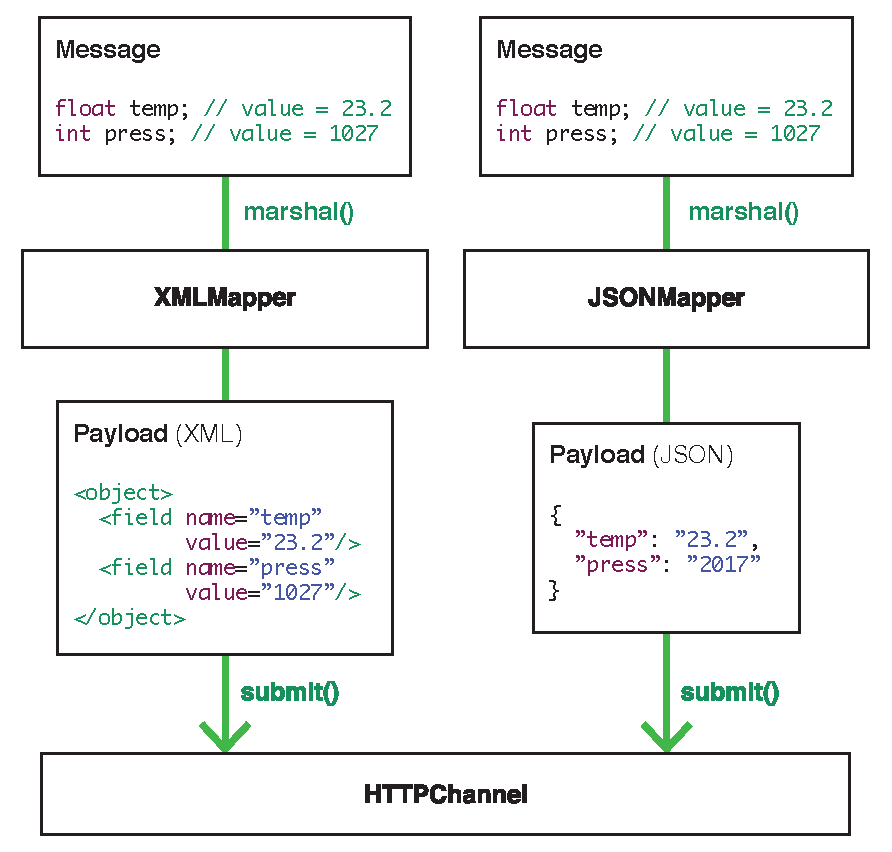
\includegraphics[scale=0.8]{imgs/mapper_channel.pdf}
    \caption{Using a single \texttt{Channel} to transmit data marshalled with
    different \texttt{Mapper}s}
    \label{fig:mapper_channel}
\end{figure}

Before this section comes to an end, it is worth putting into context the role
occupied by the \texttt{Mapper} inside the PerLa Middleware. The additional
decoupling provided by the \texttt{Mapper} builds over the pluggable
\texttt{Channel} interface, thus allowing the payload format to be selected
independently of the I/O stack.  This is an important characteristic of the
Middleware design, as even the simplest communication protocol usually requires
several \texttt{Message} structures, viz. several \texttt{Mapper}s, for
exchanging data between two endpoints.


\subsection{Creating Mappers and defining Message structures}

New \texttt{Mapper} objects are created by means of the \texttt{MapperFactory}
interface.

\lstset{language=Java}
\begin{lstlisting}[float,floatplacement=!hbt,caption=The Mapper Factory
interface,label={lst:mapperFactory}]
public interface MapperFactory {

    public Class<? extends MessageDescriptor>
        acceptedMessageDescriptorClass();

    public Mapper createMapper(MessageDescriptor descriptor,
        Map<String, Mapper> mapperMap, ClassPool classPool)
                    throws InvalidDeviceDescriptorException;

}
\end{lstlisting}

Its design follows the same concepts explained in previous sections; the
\texttt{acceptedMessageDescriptorClass()} method returns the type of
\texttt{MessageDescriptor} objects that can be used with the
\texttt{MapperFactory}, while the \texttt{createMapper()} method consumes a
\texttt{MessageDescriptor} to create a \texttt{Mapper}. However, differently
from all factory components described so far, the creation of a new object
calls for two additional parameters other than the descriptor itself: a
\texttt{ClassPool}, and a map of \texttt{Mapper}s. These extra items contain a
reference to previously built \texttt{Mapper}s, and can be used to check
whether nested \texttt{Message} fields are properly declared or not.

The \texttt{MapperFactory} interface is an additional extension point available
to PerLa users, and can be leveraged to introduce support for new binary
formats and information encoding schemes. As a consequence, every installation
of the Middleware will contain a wide variety of \texttt{MapperFactory}
implementations, each of which is dedicated to a single data format. Instances
of the previously introduced JSON and URL-Encoded mappers, for example, are
created by two distinct \texttt{MapperFactory} objects, namely
\texttt{JSONMapperFactory} and \texttt{URLEncodedMapperFactory}. This design is
a substantial improvement on the previous middleware architecture, as it
ensures that every \texttt{MapperFactory} object is responsible for managing
the quirks of only a single data format.

Moreover, every \texttt{MapperFactory} implementation is bundled with a custom
\texttt{MessageDescriptor} object, whose class name is exposed by the
aforementioned \texttt{acceptedMessageDescriptorClass()} method. The additional
complexity deriving from this design choice is more than made up for in type
safety and flexibility, as each different \texttt{MessageDescriptor} may be
implemented to closely represent the idiosyncratic characteristics of its
corresponding data format. A concrete example of this concept comes from the
\texttt{URLEncodedMessageDescriptor} class, which prevents the creation of
\texttt{Message}s that don't comply with the URL-encoded format by disallowing
non-primitive fields. Having multiple \texttt{MessageDescriptor}s also means
that different \texttt{Message}s are not forced to abide by the same set of
rules; the limits imposed on URL-encoded messages are not universal, and in
fact the \texttt{JSONMessageDescriptor} refrains from applying them.
Furthermore, \texttt{MessageDescriptor} objects can adopt a custom lexicon for
expressing the PerLa-specific concepts of \textit{message}, \textit{field} and
\textit{field type}. Take for example listings \ref{lst:jsonmessage} and
\ref{lst:urlencodedmessage}. These two XML snippets show how the vocabulary
employed in message declarations varies with the data format (field are dubbed
\textit{member} in JSON, and \textit{parameter} in URL-Encoded strings). Using
a terminology that best suits the actual data format makes \texttt{Message}
declarations idiomatic, reminiscent of the corresponding real-world objects and
therefore easier to use.

\lstset{language=XML}
\begin{lstlisting}[float,floatplacement=!hbt,caption={A compound JSON message
        declared using the JSONMessageDescriptor (XML notation). Note that the
        data type of all fields inside \texttt{weather} message is a reference
        to a previously declared \texttt{Message}.
},label={lst:jsonmessage}]

<js:object id="coord">
    <js:member name="lon" type="string"/>
    <js:member name="lat" type="string"/>
</js:object>

<js:object id="main">
        <js:member name="temp" type="float"/>
        <js:member name="pressure" type="float"/>
        <js:member name="humidity" type="float"/>
        <js:member name="temp_min" type="float"/>
        <js:member name="temp_max" type="float"/>
</js:object>

<js:object id="wind">
        <js:member name="speed" type="float"/>
        <js:member name="deg" type="float"/>
</js:object>

<js:object id="weather">
        <js:member name="coord" type="coord"/>
        <js:member name="main" type="main"/>
        <js:member name="wind" type="wind"/>
</js:object>

\end{lstlisting}


\lstset{language=XML}
\begin{lstlisting}[float,floatplacement=!hbt,caption={An URLEncoded message
declaration. Thanks to the custom \texttt{URLEncodedMessageDescriptor}, trying
to create a non-primitive field results in an exception. Note the custom
\texttt{format} attribute on the timestamp field, which is employed to define
the encoding format for dates and times},label={lst:urlencodedmessage}]

<ue:message id="urlencoded_message">
        <ue:parameter name="temperature" type="float"/>
        <ue:parameter name="pressure" type="float"/>
        <ue:parameter name="location" type="string"/>
        <ue:parameter name="key" qualifier="static" type="integer" value="5"/>
        <ue:parameter name="timestamp" type="timestamp" format="d MMM uuuu HH:mm"/>
</ue:message>

\end{lstlisting}


\subsection{Managing multiple message types}

It is not uncommon for a single device to communicate using multiple message
formats; developers may choose to encapsulate different information inside
different data structures, which the receiver must correctly identify to
decipher their contents. In such cases, every \texttt{Message} exchanged
between the two endpoints is tagged with a data type value, i.e., a common
field that advertises the type of information being transferred. This technique
is widespread among firmware developers, since it can be easily implemented
with most programming languages (C/C++ support it by design through
\texttt{tagged unions}).

The PerLa Middleware implements various techniques to cope with sensor nodes
that communicate using multiple message formats. First of all, only the data
structures that can actually be received are considered when unmarshalling a
byte stream; if under the current conditions a device only sends a subset of
its available message types, then the Middleware can immediately rule out the
unmatching ones. As it will be discussed later, a collection of expected data
formats is automatically curated by the \texttt{FPC} by cross-comparing
information excerpted from the Device Descriptor with the current device
status. It should be clear that this technique alone is not enough to cover all
practical use cases, as it falls short as soon as a device starts sending two
or more message varieties concurrenty; in such scenarios, PerLa needs to search
for clues that will help it recognize how the bytes being received are
structured. These clues take the form of \textit{static} fields. When faced
with an ambiguous situation, the \texttt{FPC} will try unmarshal the bytes
received into all expected data types. A congruency check will then be
performed on the resulting \texttt{Message}s: the data can be considered
correctly decoded only when all its static fields match the corresponding
Device Descriptor declaration. This methodology can be employed to interact
with sensor nodes that make use of tagged data structures. 


\section{Data management: Scripts}
\label{sec:components.script}

\texttt{Channel}s, \texttt{Payload}s, \texttt{Mapper}s and \texttt{Message}s
are the core components used by PerLa to exchange data with nodes of a
Pervasive System. They provide the supporting infrastructure through which
information can be serialized, transmitted and faithfully reconstructed at the
receiving endpoint. Taken together, these components implement an adaptable
transport layer, whose features can be tailored around each device connected to
the Middleware. Combine a \texttt{HTTPChannel} with a \texttt{JSONMapper} to
obtain a network stack for RESTful services; swap the data layer with an
\texttt{XMLMapper} if the format changes; add a \texttt{ZigbeeChannel} and a
\texttt{StructMapper} to communicate with low-powered devices in a mesh
network. In spite of their capabilities, all these components are not enough to
glean information from a Sensor Network. The interaction with a sensor node
requires far more than a transport layer; in fact it can only occur when data
transfer operations follow a strict set of rules, i.e., an \textit{application
protocol}. \texttt{Channel}s, \texttt{Mapper}s and \texttt{Message}s provide no
more than the basic building blocks needed for the interaction, but their use
is to be tightly orchestrated before any purposeful exchange of information can
take place.

PerLa \texttt{Script}s, just referred as \texttt{Script}s in the remainder of
this document, implement the kind of structural scaffolding required to
organize a series of primitive data management operations into a
self-contained, reusable procedure. Their purpose in the PerLa Middleware is
twofold: first, to issue commands that conform to the specific protocols used
in a Pervasive Systems; second, to act as an impedance matcher between the
structured information collected from a sensor network and the record-oriented
output of an \texttt{FPC}. The PerLa scripting language is one of the most
distinctive features of the new Middleware design; a procedural programming
tool that can be used to complement and enrich the declarative nature of the
Device Descriptor. \texttt{Script}s improve the reusability of all existing and
future Middleware components, as they can be used to adjust and adapt the
output of a computation before it is used as the input of another.



While
the former function has already been explained in the previous paragraph, the
latter needs a deeper 

PerLa script is a simple procedural programming language

\subsection{From Messages to Records}

\subsection{Available instructions}

\subsection{Engine architecture and execution model}

\subsection{Script examples}


\section{Putting it all together: the FPC}

\subsection{Data access interface}

\subsection{Controlling the remote device}

\subsection{Scheduling mechanism}


\section{Device Descriptor and FPC Factory}

\subsection{The XML Device Descriptor}

\subsection{FPC Factory}

\subsection{Registry}

\subsection{Complete XML Device Descriptor examples}
